\chapter{Format String Bugs}
\label{ch:format_string_bugs}

\begin{tcolorbox}[colback=blue!5!white,colframe=blue!75!black,title=Chapter Summary]
This chapter explores how format string functions like \texttt{printf} can be exploited when user-supplied input is directly passed as the format string. It covers the mechanisms of leaking stack memory, arbitrary memory reads, and arbitrary memory writes, culminating in full execution hijacking using staged writes.

\vspace{2mm}
\begin{center}
\begin{tabular}{|l|p{10cm}|}
\hline
\textbf{Specifier} & \textbf{Exploitation Usage} \\
\hline
\texttt{\%x} & Leaks raw values from the stack sequentially. \\
\texttt{\%N\$x} & Direct parameter access to read the $N$-th parameter on the stack. \\
\texttt{\%s} & Arbitrary read: dereferences a pointer and reads memory until a null byte. \\
\texttt{\%n} & Arbitrary write: writes the number of characters printed so far to a pointer. \\
\texttt{\%hn} & Staged arbitrary write: writes the counter as a 16-bit short integer. \\
\hline
\end{tabular}
\end{center}
\end{tcolorbox}

\section{Introduction to Format Strings}
In C and many other programming languages, printing functions often require a way to embed dynamically evaluated variables into text output. The solution to this problem is the \emph{format string}, a template containing text and special directives known as \emph{placeholders}. These placeholders tell the function how to format the data provided as subsequent arguments.

Common printing functions in C that utilize format strings include \texttt{printf}, \texttt{fprintf}, \texttt{sprintf}, and their safer variants like \texttt{snprintf}. A typical usage looks like this:

\begin{verbatim}
#include <stdio.h>
int main() {
    int i = 10;
    printf("%x %d AAA\n", i, i);
    return 0;
}
\end{verbatim}

In this snippet, the format string \texttt{"\%x \%d AAA\textbackslash{}n"} instructs the \texttt{printf} function to expect two parameters. The first parameter will be formatted as a hexadecimal integer (\texttt{\%x}), and the second as a decimal integer (\texttt{\%d}). 

Some of the most common variable placeholders are:
\begin{itemize}
    \item \texttt{\%d} or \texttt{\%i}: decimal integer
    \item \texttt{\%u}: unsigned decimal integer
    \item \texttt{\%o}: unsigned octal integer
    \item \texttt{\%x} or \texttt{\%X}: unsigned hexadecimal integer
    \item \texttt{\%c}: character
    \item \texttt{\%s}: string (expects a \texttt{char*} pointer, and prints characters until a null terminator \texttt{\textbackslash{}0} is found)
\end{itemize}

\section{The Core Vulnerability}

\begin{tcolorbox}[colback=red!5!white,colframe=red!75!black,title=Exam Insight]
A common exam task is to identify vulnerabilities in C source code. Look for functions like \texttt{printf(buf)} or \texttt{snprintf(..., buf)}, where \texttt{buf} is user-controlled. You will be asked to identify the vulnerable line, explain why it is exploitable, and propose a secure fix (e.g., rewriting it as \texttt{printf("\%s", buf)}).
\end{tcolorbox}

A format string vulnerability occurs when the format string itself is under the control of the user, rather than being hardcoded by the programmer. Consider the following seemingly harmless program:

\begin{verbatim}
#include <stdio.h>
int main(int argc, char* argv[]) {
    printf(argv[1]);
    return 0;
}
\end{verbatim}

If the user executes this program with a standard string, it behaves as expected:
\begin{verbatim}
$ ./vuln "hello"
hello
\end{verbatim}

However, what happens if the user provides a string containing format placeholders?
\begin{verbatim}
$ ./vuln "%x %x"
b7ff0590 804849b
\end{verbatim}

The \texttt{printf} function parses the format string and encounters two \texttt{\%x} placeholders. According to the C calling convention (cdecl on 32-bit x86), \texttt{printf} expects that the corresponding arguments have been pushed onto the stack by the caller prior to the function call. Since the programmer did not actually provide these arguments, \texttt{printf} blindly fetches the next values from the stack, assuming they are the intended parameters. In doing so, it unintentionally leaks the contents of the stack memory to the output.

\section{Information Leakage: Reading the Stack}

\subsection{Sequential Reading}
By providing a format string like \texttt{"\%x \%x \%x \%x"}, an attacker can sequentially pop words off the stack and inspect them. This allows an attacker to peek into the local variables of the calling function, saved return addresses, and pointers.

Moreover, if the attacker knows that the format string itself is stored on the stack (which is common for local buffers or arguments passed to a vulnerable wrapper function), they can actually read the contents of their own injected string. For instance, if an attacker provides the string \texttt{"AAAA \%x \%x \%x \%x"}, they might eventually see the hexadecimal representation of \texttt{"AAAA"} (which is \texttt{0x41414141} in little-endian ASCII) leaked in the output. This confirms that the attacker has successfully navigated the internal \texttt{printf} argument pointer back to their own controlled input.

\subsection{Direct Parameter Access}
Scanning the stack sequentially using hundreds of \texttt{\%x} placeholders can be tedious and is often limited by maximum buffer sizes. Fortunately for attackers, the POSIX standard introduces \emph{Direct Parameter Access} syntax. By using the \texttt{\%N\$x} format, an attacker can directly instruct \texttt{printf} to fetch the $N$-th parameter from the stack.

For example:
\begin{verbatim}
$ ./vuln "%3\$x"
b7fd5ff4
\end{verbatim}
This directly prints the third parameter on the stack (note that the backslash \texttt{\textbackslash{}} is used in bash to escape the dollar sign \texttt{\$}). Using direct parameter access drastically simplifies exploits, allowing an attacker to pinpoint exact offsets immediately.

\subsection{Arbitrary Read with \texttt{\%s}}
While \texttt{\%x} leaks the raw bytes on the stack, the \texttt{\%s} placeholder is far more dangerous. The \texttt{\%s} placeholder expects a \emph{pointer} to a string, and it will dereference that pointer to print memory contents until a null byte is reached.

If an attacker controls the format string and determines its offset on the stack, they can place a specific memory address directly inside the format string (e.g., \texttt{\textbackslash{}xef\textbackslash{}xbe\textbackslash{}xad\textbackslash{}xde} for \texttt{0xdeadbeef}). By using \texttt{\%N\$s} to access that exact position on the stack, \texttt{printf} will treat \texttt{0xdeadbeef} as a string pointer, fetching and printing the memory contents stored at \texttt{0xdeadbeef}. This yields an \textbf{arbitrary read primitive}, allowing the attacker to dump any readable memory in the process space. This is highly effective for bypassing memory layout randomization (ASLR) by reading the Global Offset Table (GOT) or other known structural pointers.

\section{Arbitrary Memory Write}

Information leakage is severe, but the ability to write to arbitrary memory locations elevates format string bugs to full arbitrary code execution. This is made possible by a special, often-overlooked placeholder: \texttt{\%n}.

\subsection{The \texttt{\%n} Placeholder}
Unlike other format specifiers, the \texttt{\%n} placeholder does not print anything. Instead, it expects a pointer to an integer (\texttt{int*}). It takes the \textbf{number of characters (bytes) printed so far} by the \texttt{printf} call and \textbf{writes} that number into the memory location pointed to by the argument.

\begin{verbatim}
int i = 0;
printf("hello%n", &i);
// i is now 5
\end{verbatim}

If an attacker combines the arbitrary read strategy with the \texttt{\%n} placeholder, they achieve an \textbf{arbitrary write primitive}:
\begin{enumerate}
    \item The attacker places a target memory address (e.g., \texttt{0xbffff6cc}) into the format string.
    \item The attacker uses positional arguments (\texttt{\%N\$}) to navigate to that address on the stack.
    \item Instead of using \texttt{\%s} to read, the attacker uses \texttt{\%n} to write the internal counter value to that address.
\end{enumerate}

The execution of a payload like \texttt{"\textbackslash{}xcc\textbackslash{}xf6\textbackslash{}xff\textbackslash{}xbf\%N\$n"} will cause a segmentation fault if the program attempts to write to an invalid or protected address, confirming the write primitive.

\subsection{Controlling the Written Value}
The \texttt{\%n} placeholder writes the number of characters printed \emph{so far}. To write a specific, arbitrary value, the attacker must manipulate the number of characters printed before the \texttt{\%n} is evaluated.

To write a large number, say $50,000$, the attacker does not need to inject a $50,000$-byte payload. Instead, they exploit the format specifier width padding. By using \texttt{\%50000c}, the function will print a single character padded with $49,999$ spaces, effectively advancing the internal character counter by $50,000$ using only a few bytes in the format string itself.

\subsection{Writing 32-bit Addresses in Stages}
Suppose an attacker wants to overwrite a saved instruction pointer (EIP) to hijack control flow, pointing it to a shellcode located at \texttt{0xbfffffff}. In decimal, this address is $3,221,225,471$. Using a width specifier of \texttt{\%3221225471c} would force \texttt{printf} to generate over 3 gigabytes of space padding. This would take an impractical amount of time and likely crash the application due to I/O buffering limits or timeouts.

To bypass this, attackers use the \texttt{\%hn} placeholder, which expects a pointer to a \emph{short integer} (16 bits) instead of a standard 32-bit integer. By writing the 32-bit target address in two separate 16-bit writes, the required padding drops drastically (from billions to a maximum of $65,535$).

The process involves two writes to two adjacent memory addresses:
\begin{itemize}
    \item Write the lower 16 bits of the desired payload to \texttt{TargetAddress}
    \item Write the higher 16 bits of the desired payload to \texttt{TargetAddress + 2}
\end{itemize}

Because the character counter in \texttt{printf} strictly \emph{increases}, the attacker must carefully order the two writes. The write corresponding to the \emph{smaller} 16-bit value must be executed first.

Let us assume the payload to write is \texttt{0x45434241}:
\begin{itemize}
    \item Lower 16 bits (to be written at \texttt{TargetAddress}): \texttt{0x4241} (16,961 in decimal)
    \item Higher 16 bits (to be written at \texttt{TargetAddress + 2}): \texttt{0x4543} (17,731 in decimal)
\end{itemize}

Since $16,961 < 17,731$, we write the lower half first, then print additional padding to reach $17,731$, and write the higher half.

\subsubsection{The Exploit Formula}

\begin{tcolorbox}[colback=red!5!white,colframe=red!75!black,title=Exam Insight]
Be prepared to write full exploit payloads for Format String bugs. You may need to describe each step, clearly state your assumptions, and construct the precise payload (calculating exact padding for \texttt{\%hn} writes). Furthermore, exams often require drawing the memory stack layout right before and after the format string exploit execution.
\end{tcolorbox}

\begin{figure}[h!]
\centering
% Placeholder for TikZ representation of the stack during a Format String Write
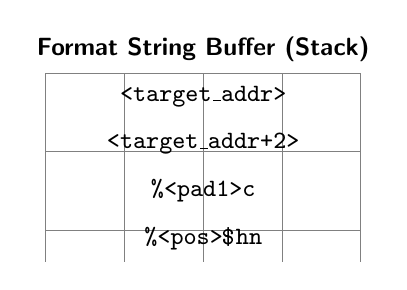
\begin{tikzpicture}[x=1cm,y=0.6cm, font=\sffamily\small]
  % Stack grid
  \draw[step=1cm,gray,very thin] (0,0) grid (4,-4);
  \node at (2,0.5) {\textbf{Format String Buffer (Stack)}};
  
  \node at (2,-0.5) {\texttt{<target\_addr>}};
  \node at (2,-1.5) {\texttt{<target\_addr+2>}};
  \node at (2,-2.5) {\texttt{\%<pad1>c}};
  \node at (2,-3.5) {\texttt{\%<pos>\$hn}};
\end{tikzpicture}
\caption{Memory layout showing the format string exploiting \texttt{\%hn} to perform a staged arbitrary write.}
\label{fig:fmt_staged_write}
\end{figure}

A generalized structure for a 16-bit-staged format string exploit looks like this (assuming the lower value is smaller than the higher value):

\begin{verbatim}
<target_addr><target_addr+2>
%<lower_value - length_of_targets>c
%<pos>$hn
%<higher_value - lower_value>c
%<pos+1>$hn
\end{verbatim}

\textbf{Handling Overflows:} If the second half is numerically smaller than the first half, the attacker relies on integer overflow. Because \texttt{\%hn} only writes the lower 16 bits, if the counter is incremented past $65,535$ (e.g., reaching \texttt{0x14241}), the \texttt{\%hn} placeholder will seamlessly write \texttt{0x4241}. Thus, the attacker simply adds $65,536$ to the smaller target value to compute the positive difference needed for the second padding.

\section{Targets for Overwriting}
With a robust arbitrary write primitive, an attacker can hijack the execution flow by overwriting key function pointers:
\begin{itemize}
    \item \textbf{Saved Return Address (Saved EIP):} Overwriting the return address on the stack. The challenge is locating the exact stack frame address reliably, making it similar to a basic stack overflow.
    \item \textbf{Global Offset Table (GOT):} A highly reliable target. The GOT stores dynamically resolved function pointers (like \texttt{exit()} or \texttt{printf()}). Overwriting a GOT entry allows the attacker to intercept subsequent library calls across the entire binary.
    \item \textbf{C Library Hooks:} such as \texttt{\_\_malloc\_hook} or \texttt{\_\_free\_hook}.
    \item \textbf{Exception Handlers:} Such as Windows SEH (Structured Exception Handling) chains.
\end{itemize}

\section{Countermeasures}

\begin{tcolorbox}[colback=red!5!white,colframe=red!75!black,title=Exam Insight]
You may be asked to analyze the bypass of memory mitigations like ASLR or Stack Canaries. A standard technique discussed in exams is using a Format String vulnerability to leak memory (such as a stack canary or a libc base address) before executing a secondary exploit like a Buffer Overflow.
\end{tcolorbox}

Modern development environments deploy several countermeasures to mitigate format string vulnerabilities:
\begin{itemize}
    \item \textbf{Compiler Warnings:} Modern compilers (\texttt{gcc}, \texttt{clang}) throw warnings (e.g., \texttt{-Wformat-security}) when a formatting function is called with a variable format string instead of a string literal.
    \item \textbf{Source Code Auditing:} Ensuring \texttt{printf(str)} is always rewritten securely as \texttt{printf("\%s", str)}.
    \item \textbf{Dynamic Mitigations:} such as \texttt{FormatGuard}, or patches to the C standard library (\texttt{libc}) that count the expected arguments and verify they match the placeholders. Furthermore, modern \texttt{libc} implementations will abort execution if the format string contains \texttt{\%n} directives and the format string resides in writable memory.
\end{itemize}

\section{Conclusion}
Format string bugs are powerful memory corruption vulnerabilities. While exploiting them requires precise mathematical calculations of offsets and paddings, the resulting exploitation provides a robust, Turing Complete arbitrary read/write primitive. By mastering direct parameter access, the \texttt{\%n} specifier, and multi-stage writes with \texttt{\%hn}, an attacker gains complete control over process execution.
